\section{Aufbau des Systems}
\subsection{Systembeschreibung}

% Bild für Systembeschreibung
\begin{figure}[htbp]
\centering 
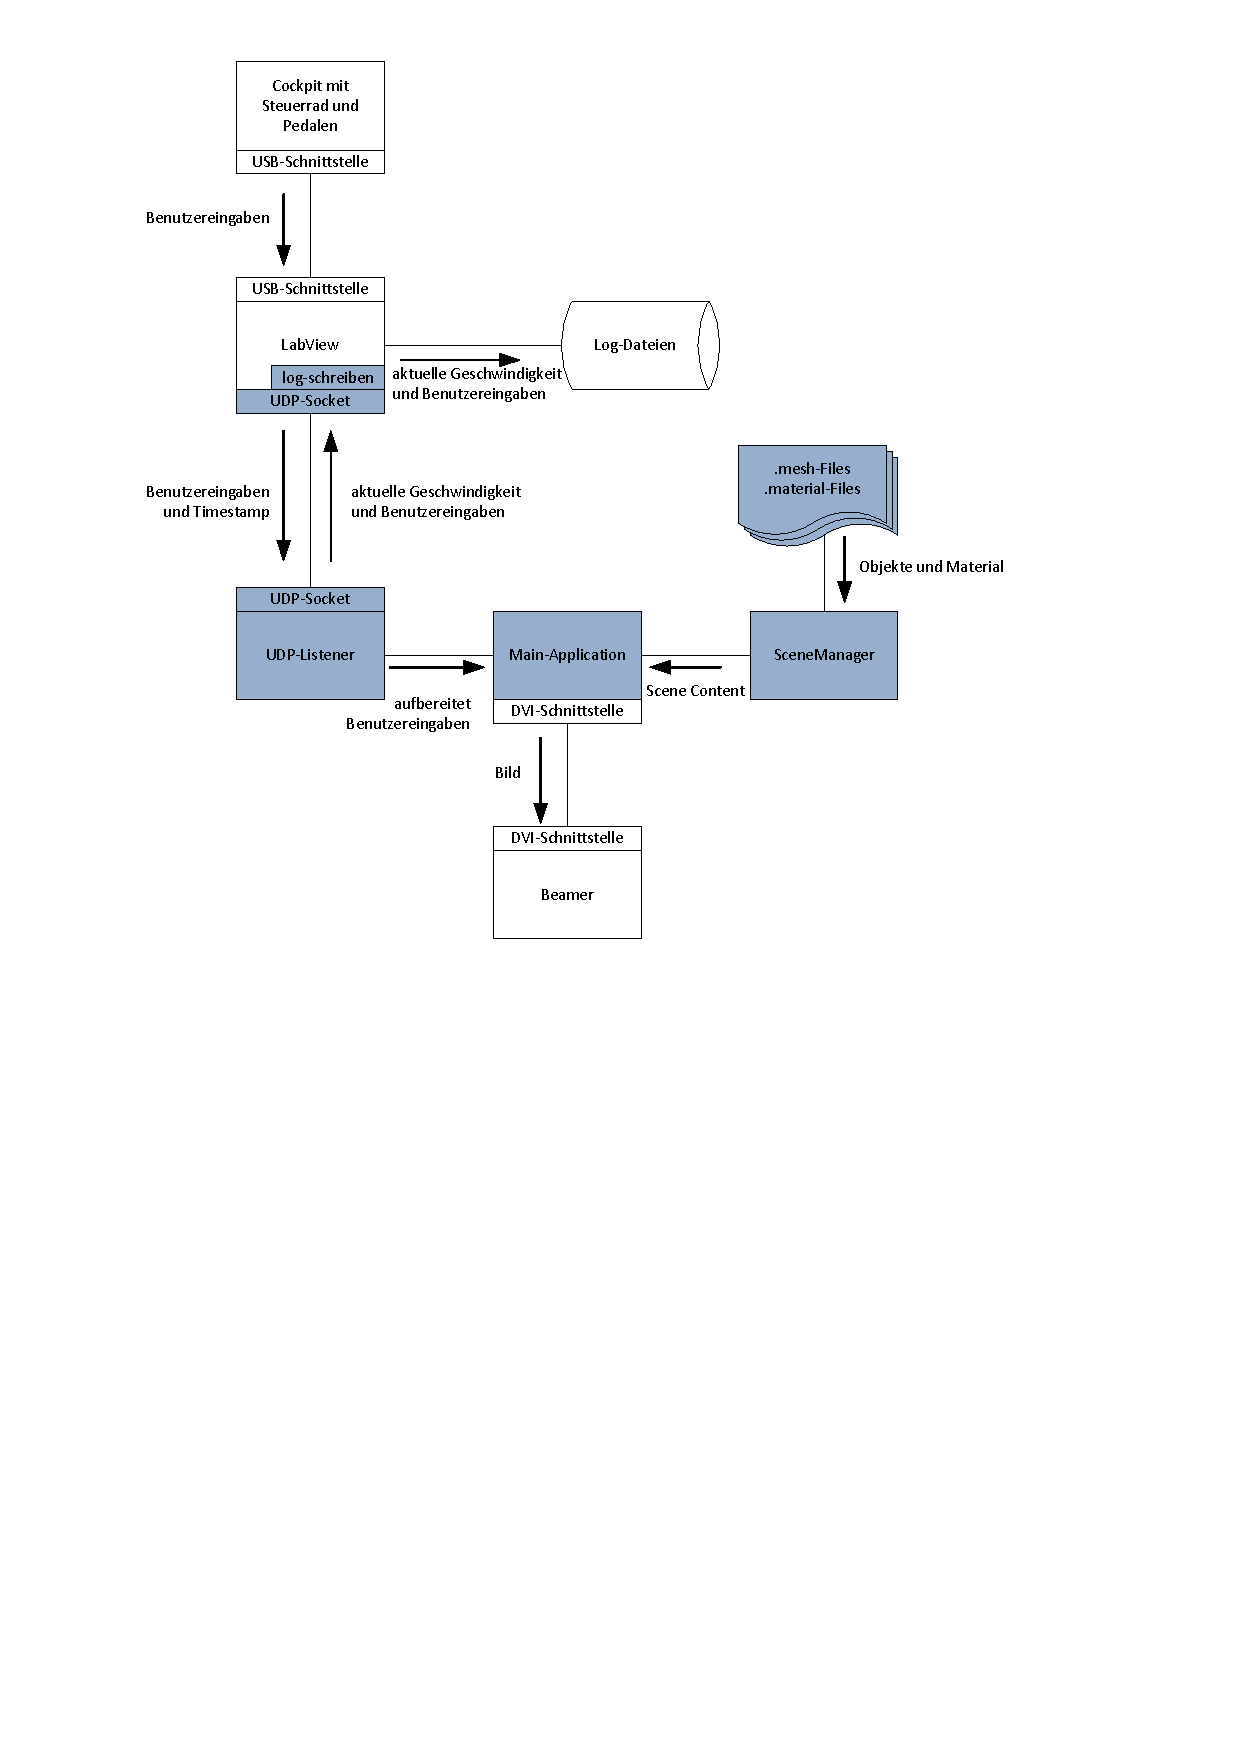
\includegraphics{src/Systembeschreibung.pdf}
\caption{Systembeschreibung} % Titel der Grafik
\label{Systembeschreibung} % Labelname
\end{figure}


Der Aufbau des Systems für den Fahrsimulator wird anhand der Abbildung \ref{Systembeschreibung} illustriert. Die blau markierten Komponenten werden im Rahmen dieser Projekt-Arbeit entwickelt. Alle übrigen sind bereits vorbestehend. \\
Benutzereingaben, die im Cockpit gemacht werden, werden von einem LabView Programm eingelesen. Nun benötigt es einen UDP-Port,  über den verschiedene Eingaben an das Programm weitergeleitet werden. Es handelt sich hierbei um Werte, die das Drehen des Steuerrades und den Druck auf Gas- oder Bremspedal quantifizieren. Zusätzlich wird der UDP-Port auch für das Empfangen diverser Log-Daten, die von unserem Programm gesendet werden, verwendet. Die empfangenen Daten werden vom LabVIEW-Programm  in ein Log-File gespeichert.\\
Weiter  muss in Programmiersprache C++ einen UDP-Socket mit entsprechendem UDP-Listener implementieren werden, um die Benutzereingaben zu empfangen. Der UDP-Listener wird gleichzeitig dazu verwendet, die Geschwindigkeit des Fahrzeugs sowie Timestamps und weitere Daten an das LabVIEW Programm zurück zu schicken. Damit können die Daten gespeichert und später ausgewertet werden.\\
Diese Aufteilung durch eine Netzwerkschnittstelle ermöglicht es,  das System, wenn notwendig, zu dezentralisieren. Einfachheitshalber wird der UDP-Listener erst in einem Video-Beispiel implementiert und getestet (Siehe Anhang B). Nachfolgend wird er in das Programm des Fahrsimulator transferiert.\\
Sind die Daten vom UDP-Listener empfangen und aufbereitet, werden sie im Hauptprogramm (Main Application) weiter verwendet. Während die Position des Steuerrades, des Gas und Bremspedales vom UDP-Listener permanent an das Hauptprogramm übertragen werden, wertet dieses die Positionen aus und veranlass die entspechenden Aktionen in der geladenen Szene. 
Die Szene selbst wird von einem Szenen-Manager geladen. Die berechnete Szene wird schlussendlich in einem Fenster von Hauptprogramm angezeigt und über eine DVI-Schnittstelle an den Beamer übertragen. Der Beamer projeziert das Bild an die Wand, die sich direkt vor dem Cockpit befindet. 

\subsection{Anforderungen}
\subsubsection{Funktionale Anforderungen}
\begin{itemize}
\item Der Fahsimulator ermöglicht es den Probanden vom Cockpit aus das Fahrzeug zu steuern. Der Porband blickt durch die Frontscheibe des Fahrzeuges und fährt auf Strassen
\item Die aktuelle Geschwindigkeit der FahzeugeVerfügung gestellt werden.  Die eine Szene stellt eine Stadt dar und die andere Szene eine Landschaft mit Tunnels.
\item Die Manipulationen des Benutzers und wichtige Parameter wie z.B. Geschwindigkeit sollen in einer Datei chronologisch und laufend abgespeichert werden um diese auszuwerten.
\item Alle ein- und ausgehenden Parameter des System sollen jederzeit in LabVIEW abrufbar sein.
\end{itemize}

\subsubsection {Nicht Funktionale Anforderungen}
\renewcommand{\labelenumi}{\alph{enumi})}

\begin{itemize}
\item Das System soll robust sein. Es muss gegen Fahlereingaben immun sein. 
\item Das Starten des Fahrsimulator sollte möglichst einfach gehalten werden.
\item Das Fahrgefühl des Simulators soll möglichst Realitätsnah sein.  
\item Der Fahrsimulator soll dem Probanden eine möglichst realistische Fahrsimulation bieten in der sich Strassen und verschiedene Objekte befinden.
\item Die Raktionszeit des Systems soll möglichst klein sein. Die Verzögerungen sollen mess-  und kalkulierbar sein.
\item Das System soll möglichst modular aufgebaut sein um später einfach erweitert werden zu können.
\item Das System soll auf der existierender Hardware funktionieren, soll aber auch noch lauffähig sein wenn Teile des Fahrsimulators ausgetauscht werden. 
\end{itemize}
